\documentclass{article}
\usepackage[utf8]{inputenc}
\usepackage{hyperref,ragged2e,amsmath,multicol,setspace,
fancyhdr,amsfonts,tikz,pgfplots,nccmath,enumerate,verbatim}
\usepackage[a4paper, width=216mm, height=297mm, margin=3cm]{geometry}
\usepgfplotslibrary{polar,fillbetween}
\usepgflibrary{shapes.geometric}
\usepgfplotslibrary{external}
\usetikzlibrary{calc,patterns,arrows}
\newcommand\mylog[1]{\mathop{{}^{#1}\mathrm{log}}}
\pgfplotsset{compat=1.15}
\pgfplotsset{my style/.append style={axis x line=middle, axis y line=
middle, xlabel={$x$}, ylabel={$y$}, axis equal }}
\usepackage{etoolbox}
\newcommand{\zerodisplayskips}{%
  \setlength{\abovedisplayskip}{0pt}%
  \setlength{\belowdisplayskip}{0pt}%
  \setlength{\abovedisplayshortskip}{0pt}%
  \setlength{\belowdisplayshortskip}{0pt}}
\pagestyle{fancy}
\fancyhf{}
\lhead{Halaman \thepage}
\rhead{Pembahasan Soal EAS 2020/2021 \\ (\href{https://instagram.com/ahmadzakiyudin_/}{@ahmadzakiyudin\_})}
\hypersetup{
    colorlinks=true,
    linkcolor=blue,
    filecolor=blue,      
    urlcolor=blue,
}
\setlength{\columnsep}{0.8cm}
\begin{document}
 \begin{titlepage}
    \vspace*{\fill}  
    \begin{center}
      \Huge {PEMBAHASAN SOAL EAS \\ MATEMATIKA II \\ TAHUN 2021/2022}\\[0.4 cm]
      \huge {Ahmad Hisbu Zakiyudin}
    \end{center}
    \vspace*{\fill}
  \end{titlepage}
\makeatletter
\renewcommand*\env@matrix[1][*\c@MaxMatrixCols c]{%
  \hskip -\arraycolsep
  \let\@ifnextchar\new@ifnextchar
  \array{#1}}
\makeatother
\newcount\arrowcount
\newcommand\arrows[1]{
        \global\arrowcount#1
        \ifnum\arrowcount>0
                \begin{matrix}[c]
                \expandafter\nextarrow
        \fi
}

\newcommand\nextarrow[1]{
        \global\advance\arrowcount-1
        \ifx\relax#1\relax\else \xrightarrow{#1}\fi
        \ifnum\arrowcount=0
                \end{matrix}
        \else
                \\
                \expandafter\nextarrow
        \fi
}
\newpage
\setstretch{1.3}
\section*{SOAL SESI 1 (Kelas 2-24)}
\begin{enumerate}
	\item Dapatkan luas permukaan dari kurva $y=\sqrt{9-x^2}, -2\leq x\leq 2$ jika diputar terhadap sumbu$-x$\\
	\textbf{Penyelesaian:}\\
	Ingat bahwa luas permukaan dari kurva $y=f(x)$ yang diputar terhadap sumbu$-x$ adalah
	$$ K=\int_a^b 2\pi f(x)\sqrt{1+[f'(x)]^2}\, dx $$
	Tinjau 
	\begin{align*}
	1+[f'(x)]^2 &= 1+\left(\dfrac{-2x}{2\sqrt{9-x^2}}\right)^2\\
	&= 1+ \dfrac{x^2}{9-x^2}\\
	&= \dfrac{9}{9-x^2}
	\end{align*}
	Batasnya yaitu $a=-2$ dan $b=2$, sehingga
	\begin{align*}
	K &=\int_{-2}^2 2\pi \sqrt{9-x^2}\sqrt{\dfrac{9}{9-x^2}}\, dx\\
	&= 2\pi \int_{-2}^2 3\, dx\\
	&= 6\pi x\big|^2_{-2}\\
	&= 6\pi [2-(-2)] = 24\pi
	\end{align*}
	\item Diberikan daerah yang dibatasi oleh kurva $y=-x^2+4$ dan sumbu-$x$
	\begin{enumerate}
		\item Sketsa daerah tersebut.
		\item Dapatkan titik berat daerah tersebut.
		\item Dapatkan volume daerah tersebut jika diputar terhadap garis $x=3$
	\end{enumerate}
	\textbf{Penyelesaian:}
	\begin{enumerate}
		\item Tinjau bahwa $y=-x^2+4$ merupakan parabola dengan titik puncak yaitu $(0,4)$, serta titik potongnya dengan sumbu$-x$ yaitu ketika $y=0$ adalah titik $(-2,0)$ dan $(2,0)$ sehingga daerahnya sebagai berikut
		\begin{center}
	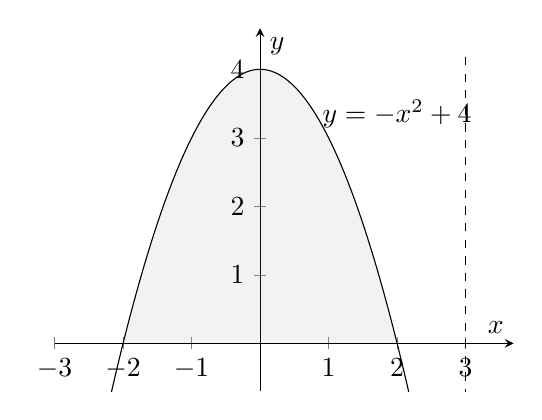
\begin{tikzpicture}
\begin{axis}[
x= 0.87 cm, y=0.87 cm,
 axis lines=middle,
  xmin=-3,xmax=3.7,ymin=-0.7,ymax=4.6,
  xtick distance=1,
  ytick distance=1,
  xlabel=$x$,
  ylabel=$y$]
\addplot[domain=-2.6:2.6,samples=300, name path=A] {-x^2+4};
\addplot[domain=-2:2,samples=300, name path=B] {0};
\draw[dashed] (3,-2) -- (3,4.2);
\draw (2,3) node[above] {$y=-x^2+4$};
\addplot[gray,opacity=0.1] fill between[of=B and A];
\end{axis}
\end{tikzpicture}
	\end{center}
	\item Perhatikan bahwa kurvanya simetris terhadap sumbu$-y$ atau garis $x=0$, sehingga $\bar{x}=0$. Selanjutnya untuk mencari $\bar{y}$ menggunakan rumus berikut
	$$
	\bar{y} = \dfrac{1}{2}\dfrac{\displaystyle \int_a^b y_1^2-y_2^2\, dx}{\displaystyle \int_a^b y_1-y_2\, dx}
	$$
	Dalam hal ini $y_1=-x^2+4$ dan $y_2$ adalah sumbu$-x$ yaitu $y_2=0$, serta $a=-2$ dan $b=2$ sehingga
	\begin{align*}
	\bar{y} &= \dfrac{1}{2}\dfrac{\displaystyle \int_{-2}^2 (-x^2+4)^2\, dx}{\displaystyle \int_{-2}^2 -x^2+4\, dx}\\
	&= \dfrac{1}{2}\dfrac{\displaystyle \int_{-2}^2 x^4-8x^2+16\, dx}{\displaystyle \int_{-2}^2 -x^2+4\, dx}\\
	&= \dfrac{1}{2}\dfrac{\displaystyle \frac{x^5}{5}-\frac{8x^3}{3}+16x\bigg|^2_{-2}}{\displaystyle \frac{-x^3}{3}+4x\bigg|^2_{-2}}\\
	&= \dfrac{1}{2}\dfrac{\frac{512}{15}}{\frac{32}{3}}\\
	&= \dfrac{1}{2}\cdot\dfrac{512}{15}\cdot\dfrac{3}{32}\\
	&= \dfrac{8}{5}
	\end{align*}
	Jadi titik beratnya yaitu $(\bar{x},\bar{y})=(0,\frac{8}{5})$
	\item Volume daerah tersebut jika diputar terhadap garis $x=3$ dapat digunakan dalil Guldin I, yaitu 
	$$ V=2\pi dL $$
	Dalam hal ini $d$ adalah jarak antara titik berat dataran dengan sumbu putar, yaitu $d=3$. Telah diperoleh pula, luas daerah tersebut yaitu $\displaystyle \int_{-2}^2 -x^2+4\, dx=\dfrac{32}{3}$. Jadi volumenya adalah $V=2\pi \cdot 3\cdot\dfrac{32}{3}=64\pi$
	\end{enumerate}
	\item Misalkan posisi suatu partikel pada saat $t$ diberikan dalam dua fungsi parametrik $x=\ln t - 1$ dan $y=\dfrac{t}{t-1}$
	\begin{enumerate}
		\item Nyatakan posisi partikel tersebut ke dalam bentuk koordinat kartesius.
		\item Gambarkan grafik lintasan partikel untuk $t\geq 2$
	\end{enumerate}
	\item Sketsa grafik daerah di luar kurva kutub $r=3$ dan di dalam kurva kutub $r=2-2\cos\theta$, selanjutnya hitung luas daerah tersebut.
	\item Diberikan fungsi $f(x)=\dfrac{1}{x^2}$
	\begin{enumerate}
		\item Dapatkan polinomial Taylor derajat 5 dari fungsi tersebut di sekitar $x=-1$.
		\item Dapatkan deret Taylor fungsi tersebut di sekitar $x=-1$ dan nyatakan dalam notasi sigma.
	\end{enumerate}
\end{enumerate}
\newpage
\section*{SOAL SESI 2 (Kelas 10-18 dan 45-61)}
\newpage
\section*{SOAL SESI 4 (Kelas 48-63)}
\begin{enumerate}
	\item Dapatkan luas permukaan dari kurva $y=|2x-4|,1\leq x\leq 3$ diputar terhadap sumbu$-x$
	\item Diberikan daerah yang dibatasi oleh kurva $y=x^2$ dan $y=4$
	\begin{enumerate}
		\item Sketsa daerah tersebut.
		\item Dapatkan titik berat daerah tersebut.
		\item Dapatkan volume daerah tersebut jika diputar terhadap garis $y=8-2x$
	\end{enumerate}
	\item Diberikan kurva kutub $r=2(1+\cos\theta),0\leq \theta\leq 2\pi$
	\begin{enumerate}
		\item Dapatkan kemiringan garis singgung pada kurva kutub tersebut di titik $\theta=\dfrac{\pi}{3}$
		\item Dapatkan semua titik $(r,\theta)$ pada kurva kutub tersebut di mana garis singgungnya vertikal.
	\end{enumerate}
	\item Sketsa grafik daerah di dalam kurva kutub $r=6\sin\theta$ dan di luar kurva kutub $r=2+2\sin\theta$, selanjutnya hitung luas daerah tersebut.
	\item Diberikan fungsi $f(x)=e^{-x}$
	\begin{enumerate}
		\item Dapatkan polinomial Maclaurin derajat 5 dari fungsi tersebut
		\item Dapatkan deret Maclaurin fungsi tersebut dan nyatakan dalam notasi sigma.
	\end{enumerate}
\end{enumerate}
\end{document}
